We assume that there is a "Theory of Everything", called ToE herein, which is suspected to include a contained description of small and large scale forces in the universe (e.g., strong nuclear, weak nuclear, electromagnetic, and gravitational forces). Our classical observations fall into a low energy, large scale, decoherent approximation of this ToE. The purpose of this collection of notes is to study \textit{(effective) relativistic quantum field theory} which is the low energy, large scale approximation of the ToE, and we are not sure how many "steps" there are in between the two, but the relativistic quantum field theory is the closest we currently come to a ToE. If we lower the energy and lengthen the scale of our study, we land in a nonrelativistic quantum field theory. A quantum field theory is then subject to decoherence, as we exist on the classical scale, and we begin the development of a relativistic quantum field theory with a classical field theory. In this sense, our purpose is to undo all of the approximations that nature forces us to take when we run experiments, take measurements, and devleop theoretical frameworks to describe observed phenomena.

\begin{figure}[H]
	\centering
	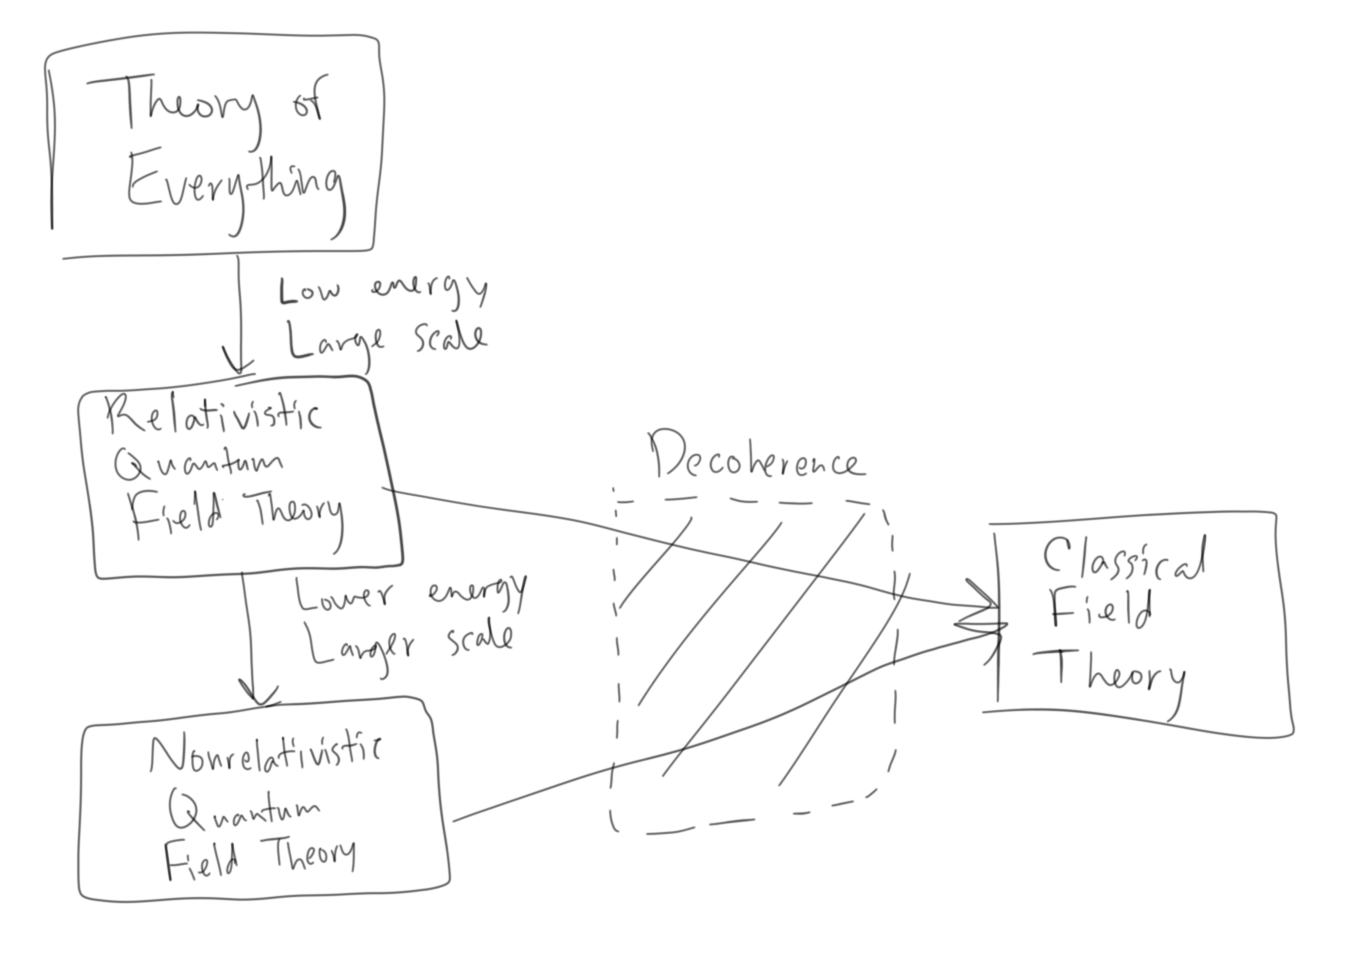
\includegraphics[width=\linewidth]{toe.png}
	\caption{Schematic of the study of field theories in physics.}
	\label{fig:fig1}
\end{figure}

\clearpage

\subsection*{Mathematical Machinery of Relativistic QFT}

For a quantum field theory to be relativistic it must be symmetric under the Poincar\'e group transformations.

\noindent Let the four-vector $(x_0, x_1, x_2, x_3)$ be the spacetime coordinates in an inertial reference frame. Then in any other reference frame that an observer chooses, the following condition is satisfied. 

\noindent (Note: We adopt the Einstein summation notation, and repeated indices are summed over, such that $\mu$, $\nu$, $\rho$, and $\sigma$ below are summed from $0$ to $3$.)

\begin{equation}
\eta_{\mu\nu} dx'^\mu dx'^\nu = \eta_{\rho\sigma} dx^\rho dx^\sigma
\end{equation}

\noindent Where we are using the Minkowski metric
\begin{equation}
\eta_{\mu\nu} 
= g_{\mu\nu} 
= \left( \begin{array}{rrrr} 
1 & 0 & 0 & 0 \\ 
0 & -1 & 0 & 0 \\ 
0 & 0 & -1 & 0 \\ 
0 & 0 & 0 & -1 
\end{array} \right)
.
\end{equation}

\noindent Any transformation satisfying the first equation, the relationship between the coordinates of two reference frames, must be a \textit{linear transformation} of the form, denoted by the pair $(\Lambda, a)$,
\begin{equation}
x'^\mu = \Lambda^\mu_{\,\,\,\nu} x^\nu + a^\mu
\end{equation}

\noindent Where $\Lambda^\mu_{\,\,\,\nu}$ is the $4x4$ Lorentz transformation matrix that represents rotations, and $a^\mu$ is a constant four-vector that represents spatial translations. 

\noindent Also note that the Lorentz transformation must satisfy the following condition, shown in index and matrix notation.
\begin{align}
	\eta_{\mu\nu} \Lambda^\mu_{\,\,\,\rho} \Lambda^\nu_{\,\,\,\sigma} &= \eta_{\rho\sigma} \\
	\Lambda^{T} \eta \Lambda &= \eta
\end{align}

\noindent These transformations $(\Lambda, a)$ are the elements of the Poincar\'e group $\mathcal{P}_4$. Let's check the group conditions, using equation \eqref{eq:eqn2} for calculating the product of two Poincar\'e transformations,

\begin{equation}
\begin{array}{llll} 
product & (\Lambda, a) \circ (\bar{\Lambda}, \bar{a}) & = & (\bar{\Lambda} \Lambda, \bar{\Lambda} a + \bar{a}) \\ 
identity & (1, 0) \circ (\Lambda, a) & = & (\Lambda, a) \\ 
inverse & (\Lambda^{-1}, a^{-1}) \circ (\Lambda, a) & = & (1, 0) \\ 
associativity & \left( (\Lambda, a) \circ (\bar{\Lambda}, \bar{a}) \right) \circ (\bar{\bar{\Lambda}}, \bar{\bar{a}}) & = & (\Lambda, a) \circ \left( (\bar{\Lambda}, \bar{a}) \circ (\bar{\bar{\Lambda}}, \bar{\bar{a}}) \right)
\end{array}
\end{equation}

\noindent In index notation, the total effect of the product of two Poincar\'e transfomations is written as
\begin{align}
x'^\mu &= \Lambda^\mu_{\,\,\,\nu} x^\nu + a^\mu \\
x''^\mu &= \bar{\Lambda}^\mu_{\,\,\,\rho} x'^\rho + \bar{a}^\mu
\end{align}

\noindent Quantum mechanical symmetries are representated by \textit{unitary} or \textit{anti-unitary} linear operators as elements of a separable Hilbert space $\mathscr{H}$ such that for each Poincar\'e transformation $(\Lambda, a) \in \mathcal{P}_4$, there exists a unitary transformation 
\begin{equation}
U(\Lambda, a) : \mathscr{H} \rightarrow \mathscr{H}
\end{equation}

\noindent The identity unitary transformation, and the product of any two unitary transformations of elements of the Poincar\'e group are physically indistinguishable from each other up to a phase factor $e^{i\phi}$, where $\phi \in \mathbb{R}$
\begin{align}
U(\bar{\Lambda}, \bar{a}) U(\Lambda, a) &= e^{i\phi((\Lambda, a),(\bar{\Lambda}, \bar{a}))} U(\bar{\Lambda} \Lambda, \bar{\Lambda} a + \bar{a}) \\
U(\mathbbm{1}, 0) &= e^{i\phi} \mathbbm{1} .
\end{align}

\noindent The family of transformations $U(\Lambda, a)$ that satisfy these equations is called the \textit{projective unitary representations of} $\mathcal{P}_4$, and is precisely what we need to establish a relativistic quantum field theory that includes translations, rotations, and Lorentz boosts as its transformations.\\

\noindent Consider the \textit{time translation subgroup} of the Poincar\'e group 
\begin{equation}
\{ (\Lambda=\mathbbm{1}, a=(t, 0, 0, 0)): t \in \mathbb{R} \} \subset \mathcal{P}_4
\end{equation}
\noindent And let $U$ be a unitary representation of $\mathcal{P}_4$. Then $V(t) = U(\mathbbm{1}, (t, 0, 0, 0))$ is a one-parameter family of unitary transformations, which is a group homomorphism, such that $V(s)V(t)=V(s+t)$, and is called a \textit{propagator}, and is a solution to the Schr\"{o}dinger equation, assuming the Hamiltonian $\hat{H}$ is self-adjoint and is stable, such that there at most a finite number of, preferrably zero, negative eigenvalues

\begin{equation}
\frac{d V(t)}{dt} = i \hat{H} V(t).
\end{equation}

\noindent So, having a unitary representation is equivalent to solving the time-dependent Schr\"{o}dinger equation, and we require that $U(\Lambda, a)$ is positive energy, such that the spectrum of eigenvalues of $\hat{H}$ is positive $spec(\hat{H}) \subset \mathbb{R}^+$, and stable. Otherwise, the system may be unstable and plunge to more and more negative eigenvalues. \\

\noindent All single-particle unitary representations of $\mathcal{P}_4$ have been classified by Wigner, and are labelled by their mass $m$ (invariant under Poincar\'e and Lorentz transformations) and their helicity/spin $s$. The bad news is that the universe is comprised of many particles, creating tension between locality and interactions, rendering thorough study of single-particle representations pointless. Even for a single particle, as we increase locality, self-interaction increases, and new particles are created via tunnelling. \\

\subsection*{Why is Obtaining a Relativistic Quantum Field Theory Hard?}

\noindent The reason that constructing a relativistic QFT is considered so difficult is because there are no nontrivial, only trivial, finite-dimensional unitary representations of the Poincar\'e group $\mathcal{P}_4$. The only nontrivial representations of $\mathcal{P}_4$ are infinite-dimensional, and are not easy to work with when constructing a unitary representation. Consider this in contrast to the, more easily constructed, special orthogonal group of three-dimensional rotations $SO(3)$ with unitary representations 

\begin{equation}
U = e^{i(\sigma_x \hat{J}_x + \sigma_y \hat{J}_y + \sigma_z \hat{J}_z)}. 
\end{equation}

\noindent Where $\hat{J}_\alpha$ are the angular momentum operators. The reason $SO(3)$ is easier to work with and construct a unitary representation is because $SO(3)$ a \textit{compact} group, while $\mathcal{P}_4$ is a \textit{non-compact} group.